% @Author: AnthonyKenny98
% @Date:   2020-04-10 06:34:08
% @Last Modified by:   AnthonyKenny98
% @Last Modified time: 2020-04-10 08:06:42
\begin{figure}[H]
\begin{center}
\begin{tabular}{cc}


\begin{subfigure}{0.3\textwidth}
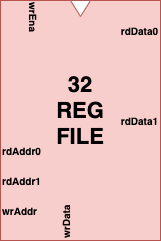
\includegraphics[width=\linewidth]{chapters/chapter4/img/regfile1.png}
\caption{}
\label{fig:regfile1_a}
\end{subfigure}

\begin{subfigure}{0.3\textwidth}
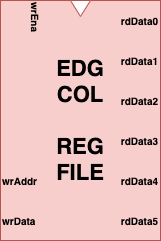
\includegraphics[width=\linewidth]{chapters/chapter4/img/regfile2.png}
\caption{}
\label{fig:regfile1_b}
\end{subfigure}

\end{tabular}
\mycaption{PhilosophyV Register Files}{. Figure \ref{fig:regfile1_a} shows the 32RVI register file, containing 32 registers. The ports \texttt{readData0} and \texttt{readData1} output the data held at the address provided to  \texttt{rdAddr0} and \texttt{rdAddr1} respectively. Figure \ref{fig:regfile1_a} shows the Xedgcol register file, which is able to constantly output all 6 values held within it. Since the Xedgcol ISA only defines their use for one instruction, these ports can be wired directly to the HoneyBee unit.}
\label{fig:regfiles}
\end{center}
\end{figure}